\documentclass[11pt]{article}

\usepackage{amsmath}
\usepackage{graphicx}

\begin{document}
    \title{DoH water torture attack}
    \date{}
    \maketitle

    \section{DNS water torture attack}
    DNS water torture attack (aka. [Pseudo-]Random subdomain attack) is a DDoS attack that floods authoritative servers with randomly generated DNS queries.
    Usually the attacker orchestrate the attack using a C2 server and a botnet consisting of numerous compromised devices.
    These devices generate random subdomains of the target domain and try to query their corresponding IP address using DNS. Since these DNS queries are virtually distinct, they undermine the DNS caches in the network and flood the authoritative nameserver(s) of the victim, wasting resources and potentially affecting availability of the DNS service.
    Recursive nameservers along the way are also prone to receive collateral damage.

    \section{Implications of DoH protocol}

    DoH protocol may affect this attack in different ways.
    First of all, DoH protocol can be implemented in different settings and it is important to acknowledge the role of DoH in water torture attack in each of these settings.

    \subsection{Bots connecting to DoH server directly}

    If bots connect to the DoH server to send their flood of queries, all of the traffic between them would be encrypted.
    To mitigate such attacks, network administrators may wish to block DoH flows completely.

    The encrypted traffic make detection of this attack in local networks (such as IoT gateways) harder.
    On the other hand, since clients need to connect to the DoH server first, a reputation system for sessions might be useful in mitigating the attack.
    Fingerprinting techniques are also an interesting candidate for detection of malicious clients.

    \begin{figure}[h]
        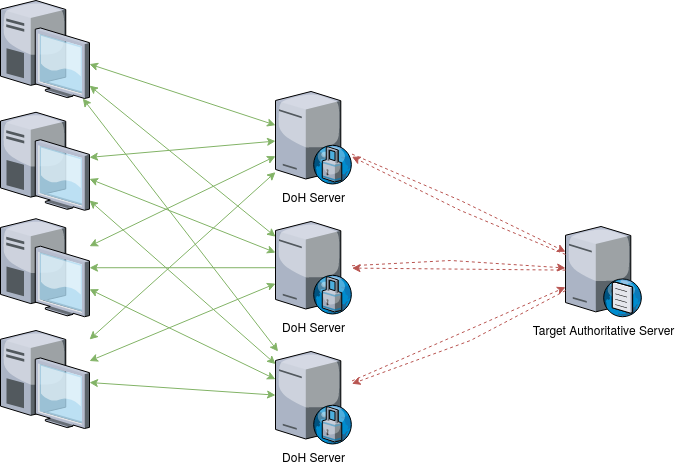
\includegraphics[width=10cm]{direct.png}
        \caption{Connecting directly to the DoH server}
    \end{figure}

    \subsection{Bots connecting to DoH through DoH Proxy}

    In the second setting, clients (including the malicious ones) use traditional DNS to communicate with a DoH proxy that resolves the queries by using DoH protocol.
    In this scenario, the local network and the DoH proxy can serve as detection and mitigation points, since the DNS traffic is still available for analysis.

    Using these approach, either happening by chance or mediated by the attacker, malicious clients can use legitimate sessions used by all other benign clients to circumvent detection methods based on reputation of clients.

    \begin{figure}[h]
        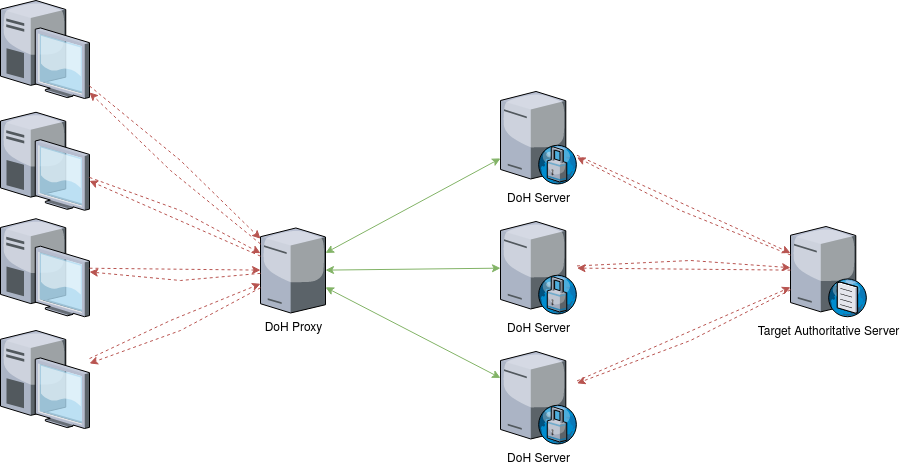
\includegraphics[width=\textwidth]{proxied.png}
        \caption{Connecting to the DoH server through the DoH proxy}
    \end{figure}

    \section{Attack scenario}

    To simulate a DoH water torture attack, we need to first create a network having both of the mentioned settings for deploying DoH. This network includes a DoH server, a DoH proxy, any number of DoH-enabled clients connecting directly to the server, and any number of traditional clients connecting to DoH server through the DoH proxy.
    Each of these clients use a portion of a host name dataset to collectively simulate the baseline name resolution activity in a network.

    Furthermore, any number of malicious clients will be added to the network, all trying to flood the authoritative server of ``targetdomain.site`` by performing a random subdomain attack.
    These clients may be DoH-enabled clients directly communicating with DoH server, or traditional clients behind a DoH proxy.
    Figure~\ref{fig:attack} shows the network used in this attack scenario.
    \begin{figure}[h]
        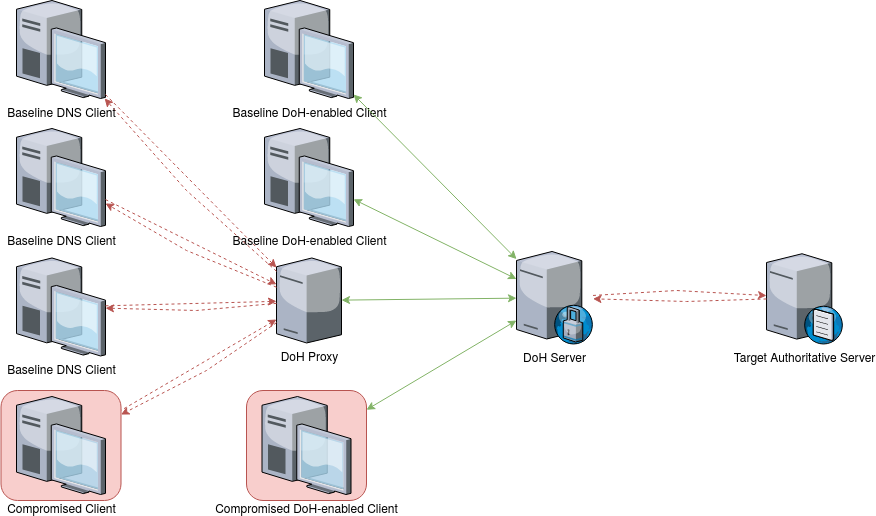
\includegraphics[width=\textwidth]{attack.png}
        \caption{Attack scenario network}
        \label{fig:attack}
    \end{figure}

    \section{Mitigation}
    To mitigate these attacks we introduce a design for DoH servers to detect potential malicious requests and alleviate the attack while maintaining low collateral damage to the legitimate clients (false positives).
    We can use statistics from the DNS zones (such as number of recent NXDOMAIN and SERVFAIL responses) to schedule the ongoing DNS recursion made by this server when a cache miss occurs.
%    By changing the priorities of these request, we can prevent this server acting as a
    Figure~\ref{fig:mitigate} shows the mitigation technique.
    \begin{figure}[h]
        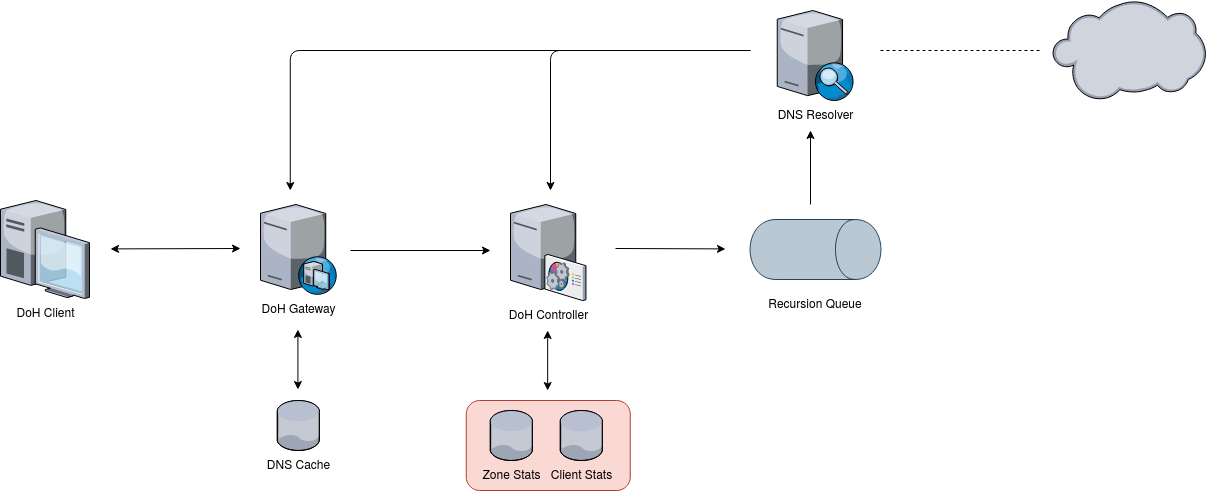
\includegraphics[width=\textwidth]{mitigation.png}
        \caption{mitigation technique}
        \label{fig:mitigate}
    \end{figure}

\end{document}